\section{Tolerating Lack of Connectivity}
\label{unlinkable-design-3}

Both the Basic and the Secure Unlinkable CC Protocols suffer from requiring ready access to the Internet.
Each transaction requires the virtual credit card to acquire a new token \emph{T} from the Wallet Server.
As such, lack of connectivity (e.g. paying for parking in an underground garage, making purchases while in a foreign country, etc) significantly hampers the ability for
    customers to use their credit cards.
This can be alleviated somewhat by requesting multiple tokens at once, but remains a fundamental limitation of the protocols.

In this third protocol (termed simply the Unlinkable CC Protocol), we solve this problem by generating the single-use tokens within the Wallet Application.
Tokens are generated deterministically and using information available to both the Wallet Server and Wallet Application.
As a result, both the Wallet Application and Wallet Server are able to independently generate the same tokens for a given card without needing to communicate.
Communication between the Wallet Application and the Wallet Server is no longer necessary besides during card registration (and resolution to synchronization problems).

As before, when the Wallet Server receives a Registration message, it stores the card information and associates a card identifier \emph{Ident} with this record.
It also generates a secret key \emph{secret} associated with this card.
In the Unlinkable CC Protocol, the Wallet Server responds to the Registration message with this identifier \emph{Ident} and the key \emph{SK}.
The Wallet Application stores these values securely, associating them with the credit card being registered.

Both the Wallet Application and the Wallet Server initialize a transaction counter for this card, and set it to zero.
In addition, the Wallet Server calculates the initial token \emph{T}, by calculating the keyed hash of the transaction counter (currently at 0) keyed with key \emph{SK}.
The Wallet Server stores this initial value of \emph{T} with the credit card record.
The protocol, illustrated in Figure \ref{fig:unlinkable-3}, operates as follows:

\begin{figure}[h!]
  \caption{Unlinkable CC Protocol}
  \centering
    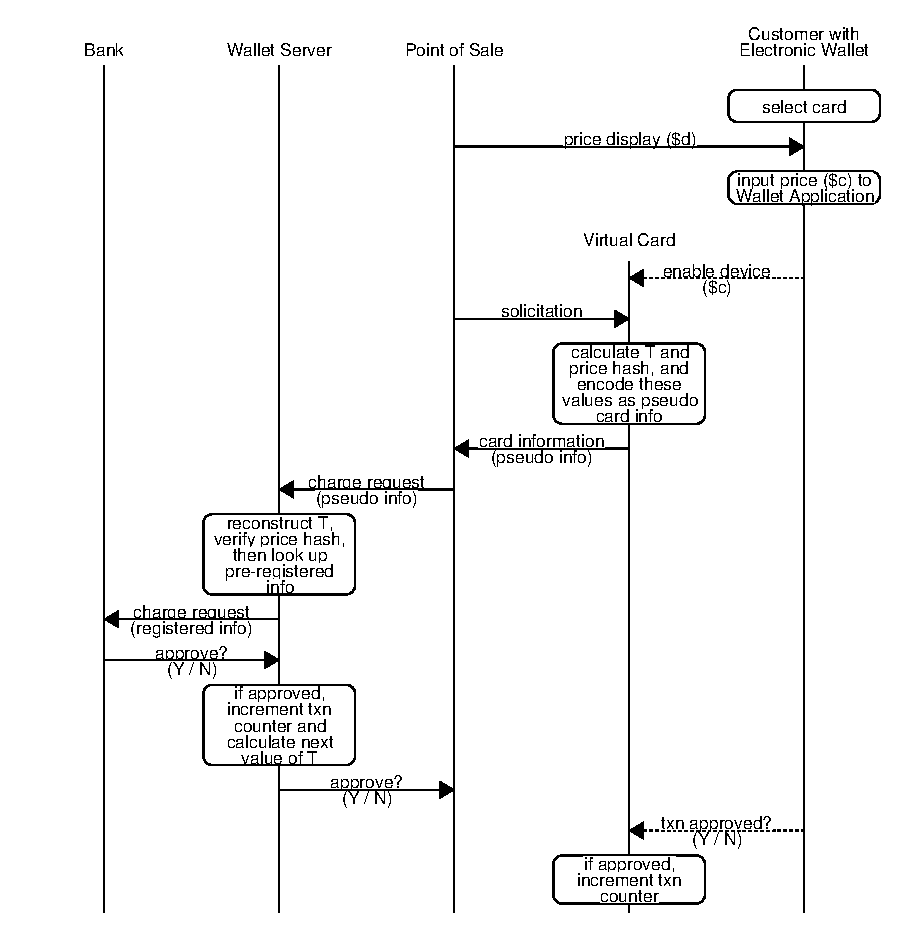
\includegraphics{img/unlinkable-3.eps}
  \label{fig:unlinkable-3}
\end{figure}

\begin{enumerate}
\item When the customer wishes to use a credit card, the customer selects a credit card in the Wallet Application.

\item The point of sale displays the price to charge (\$d) on its screen.

\item The customer enters the price to be charged (\$c) into the Wallet Application.

\item The Wallet Application now enables the virtual credit card, initializing it with price \$c.
    The virtual credit card begins listening for Solicitation messages.

\item The point of sale sends a Solicitation message to the virtual credit card over the NFC channel.

\item
    The virtual credit card calculates token \emph{T} by hashing the transaction counter keyed with the key \emph{SK}, and selecting the first 80 bits.
    The virtual credit card then proceeds as before.
    It calculates the price hash as before, by combining \emph{T} with price \$c,
        hashing this value with key \emph{SK}, and selecting the first 13 bits.
    It then combines the 80-bit token \emph{T} with this 13-bit price hash to acquire a 93-bit value.
    Finally, it converts this 93-bit value into a 28-digit number \emph{k}, and responds with a pseudo Card Information message as before.

\item The point of sale constructs an Charge Request message from the (pseudo) Card number, Expiration date, iCVV, and the price it wishes to charge.
    This message is sent to the bank named in the Card Information message.
    As a result, the Charge Request message is directed to the Wallet Server and \emph{not} an actual bank.
    Note that from the perspective of the point of sale, the Wallet Server appears to be a bank like any other.

\item The Wallet Server reconstructs \emph{k} from the Charge Request message, and computes the 80-bit token and 13-bit price hash that it represents.
    The Wallet Server then searches its database for the token, to identify the card used in this transaction.
    If exactly one token is not found, the Wallet Server sends a ``declined'' Acceptance message to the point of sale, and aborts the protocol.
    Otherwise, the secret key \emph{SK} is retrieved from the Wallet Server's database, and the Wallet Server calculates its own version of the price hash
        using the price indicated by the point of sale in the Charge Request message.
    If the Wallet Server's price hash does not match the price hash in the Charge Request mesage,
        the Wallet Server sends a ``declined'' Acceptance message to the point of sale and aborts the protocol.
    Otherwise, the stored card information is retrieved from the Wallet Server's database.
    The Wallet Server sends a \emph{visual} Charge Request to the card's bank with the following fields:
    \begin{itemize}
    \item Cardholder name
    \item Card number
    \item Expiration date
    \item Billing address
    \end{itemize}
    Note that unlike the Card Information message sent by the Wallet Application, this data reflects the actual credit card information,
        acquired by the Wallet Server during the card registration.

\item The bank receives the \emph{visual} Charge Request from the Wallet Server, and processes this transaction as normal.
    The bank then responds to the Wallet Server with an Acceptance message indicating whether the charge has been accepted.

\item The Wallet Server examines the Acceptance message from the bank.
    If the charge was accepted, it increments the transaction counter associated with the virtual credit card, and recalculates the next expected value of \emph{T}.
    The Wallet Server then forwards the bank's Acceptance message to the point of sale.

\item The Wallet Application prompts the customer as to whether the charge was accepted by the bank.
    Note that the Acceptance message is not sent to the Wallet Application or virtual credit card as part of the protocol,
        and so the Wallet Application must rely on the customer to enter this data.
    If the charge was approved, then the virtual credit card increments its transaction counter.
\end{enumerate}

The Unlinkable CC Protocol is identical to the Secure Unlinkable Protocol,
    with the exception that the tokens \emph{T} are generated independently in both the Wallet Application and the Wallet Server.
As a result of this change, there are two potential failure cases which must be considered.

First, since the protocol relies on the customer manually maintaining the transaction counter within a virtual credit card,
    we must account for potential customer error.
If a customer fails to increment the transaction counter on a successful purchase (or incorrectly increments it on a failed purchase),
    then the Wallet Server and the virtual credit card will not agree on subsequent values of \emph{T}.
The transaction counter can be re-synchronized by way of an authenticated message exchange with the Wallet Server, sent securely over the Internet.
As such, customer error in maintaining a virtual credit card's internal transaction counter results in an inoperative virtual credit card
    until such a time as the Wallet Application regains temporary access to the Internet.

Second, since the Wallet Server can no longer exercise full control over token generation, we must consider the possibility of token collisions.
A token collision occurs when two different virtual credit cards calculate the same token \emph{T} at the same time.
This occurs when \emph{H(SK\textsubscript{1}, txn\_ctr\textsubscript{1}) = H(SK\textsubscript{2}, txn\_ctr\textsubscript{2})}.
The resolution is similar: both virtual cards become inoperative until \emph{at least one} of the corresponding Wallet Applications regains access to the Internet
    and negotiates a new transaction counter\footnote{
    We refer to the value as a ``transaction counter'' because we increment it with every transaction,
        but there is no requirement that it reflect an accurate number of transactions.
    It need only be a value which (a) changes on every successful transaction, and
        (b) changes in such a way that both the Wallet Application and Wallet Server can independently agree on the new value.
    As such, resolution to a collision consists simply of incrementing the transaction counter of whichever card is first to reconnect to the Internet, and resynchronizing.
    }.
Note however that the probability of such a collision is negligibly small, and will be examined in Chapter \ref{cha:simulation}.